%-------------------------------------------------------------------------------
% Preamble
%-------------------------------------------------------------------------------

\documentclass{article}


%Packages
\usepackage{
	siunitx, % units
  graphicx, % for images
	natbib,
	booktabs
}
\usepackage[letterpaper]{geometry}
\renewcommand{\thefigure}{S\arabic{figure}}
\renewcommand{\thetable}{S\arabic{table}}
\usepackage[breaklinks=true]{hyperref}


%-------------------------------------------------------------------------------
% Title and Authors
%-------------------------------------------------------------------------------

\title{Supplemental Information for\\``Extreme rainfall in Paraguay during the 2015-2016 austral summer: causes and subseasonal-to-seasonal predictive skill''}
\author{James Doss-Gollin\and \'{A}ngel G. Mu\~{n}oz \and Simon J. Mason \and Max Past\'{e}n}
\date{\today}

\begin{document}

%% Necessary!
\maketitle

This document contains several supplemental figures described in the main text.
Further supporting information is available in the form of source code and \texttt{jupyter} notebooks at \url{github.com/jdossgollin/PYFloods}.

\listoftables
\listoffigures

\clearpage

\begin{table}
	\centering
	\begin{tabular}{lrr}
		\toprule
		{} &  NDJF 2015-16 &  Climatology \\
		WT &           &              \\
		\midrule
		1     &  0.266667 &     0.213306 \\
		2     &  0.216667 &     0.177793 \\
		3     &  0.133333 &     0.160935 \\
		4     &  0.116667 &     0.152619 \\
		5     &  0.191667 &     0.151944 \\
		6     &  0.075000 &     0.143403 \\
		\bottomrule
	\end{tabular}
	\caption{Weather type (WT) occurrence fraction during NDJF 2015-16 and Climatology}
\end{table}

\clearpage

\begin{figure}
	\centering
  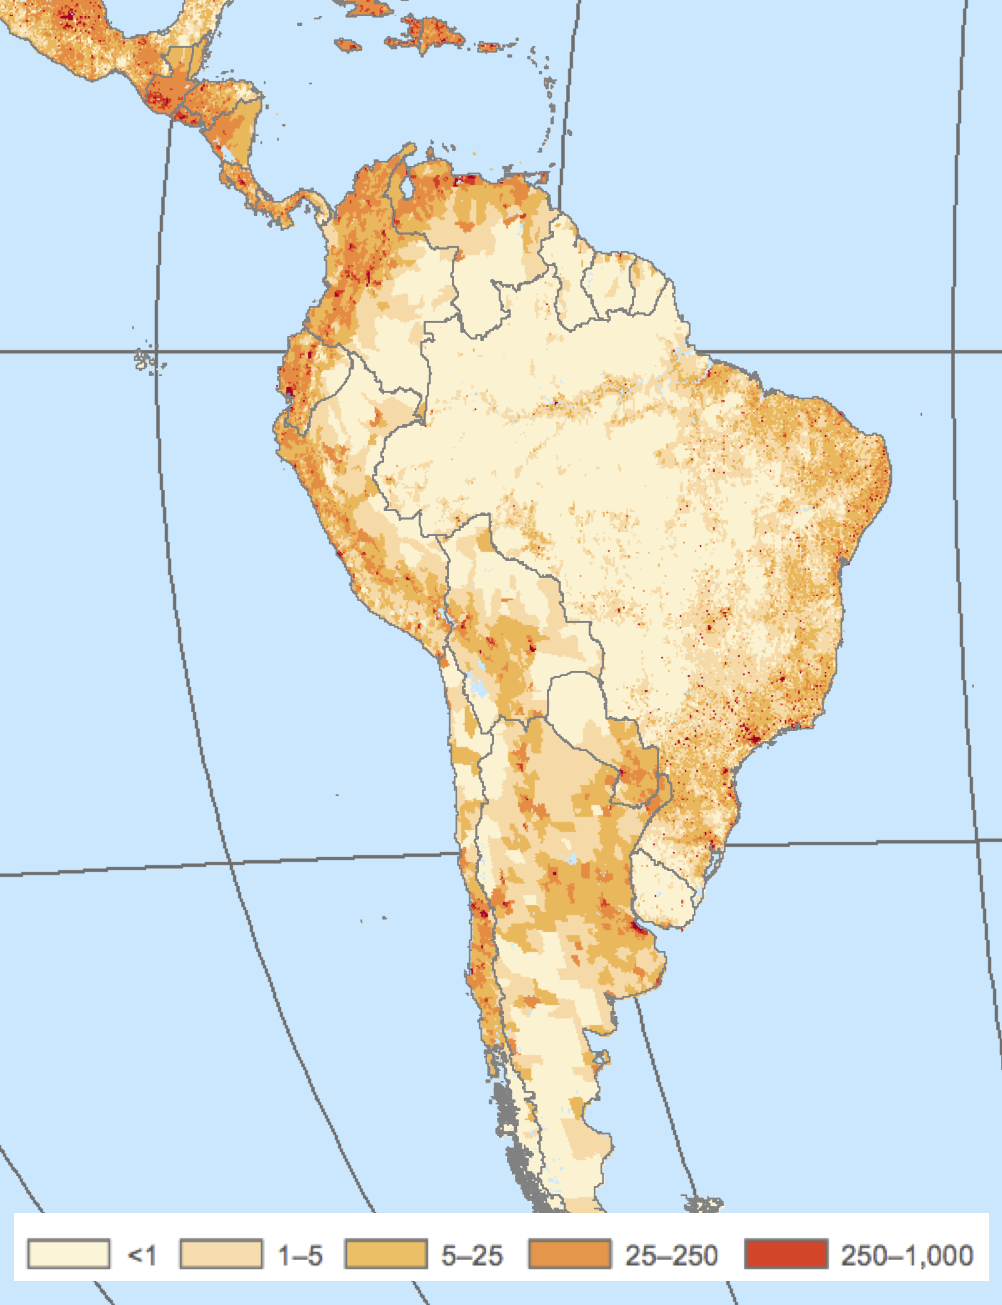
\includegraphics[width=\textwidth,height=0.9\textheight,keepaspectratio=true]{gpw-v4-2015.png}
	\caption{
		Gridded estimate of population density (color; in units of persons per square kilometer) from \citet{GPWv4}.
	}
\end{figure}

\begin{figure}
  \includegraphics[width=\textwidth]{../figs/PSI_Var_Explained.pdf}
	\caption{
		Variance explained for each EOF loading of the \SI{850}{\hecto\pascal} streamfunction $\psi$.
    (L): the individual variance explained for each EOF.
		(R): cumulative variance explained.
	}
\end{figure}

\begin{figure}
  \includegraphics[width=\textwidth]{../figs/WT_Classifiability.pdf}
	\caption{
		Classifiability index \citep[see Methods and][]{Michelangeli1995} calculated for several chosen values of $K$, representing the number of weather types produced.
		Results are produced with only 50 simulations for each $K$.
	}
\end{figure}

\begin{figure}
  \includegraphics[width=\textwidth]{../figs/knn_rainfall_EOF.pdf}
	\caption{
    Expected rainfall over two regions conditional on the (simultaneous) values of EOF2 and EOF3 of the \SI{850}{\hecto\pascal} streamfunction $\psi$ shown in the main text.
    The ``Chaco Jet Extension Region'' is defined as extending from \SIrange{299.25}{302.75}{\degree E} and \SIrange{34.75}{30.75}{\degree S} and the ``Lower Paraguay River Basin'' is defined in the main text.
    Both values represent area-averaged rainfall time series.
    Expected rainfall is calculated by using a nearest-neighbors regression with 100 neighbors in the two-dimensional phase space of EOF2 and EOF3.
    Because nearest-neighbors approaches tend to perform poorly under extrapolation (where there are few observations), the domain shown is limited to regions with high density of observations.
  }
\end{figure}

\begin{figure}
  \includegraphics[width=\textwidth]{../figs/ENSO_MJO_EOF_PRCP_Time_Series.pdf}
	\caption{
		Time series of S2S predictors and their influence on evolution of circulation and rainfall.
    Top row shows two predictors shown to influence the circulation: monthly NINO3.4 index and daily MJO RMM1 index.
    Blue dots show daily observations of MJO RMM1, while the blue line shows the MJO RMM1 time series with a 7-day rolling mean applied.
    Bottom row shows the evolution of EOFS 2 and 3 of the \SI{850}{\hecto\pascal} field.
    As for the MJO RMM1, dots show the daily fields and lines show the fields with a 7-day running mean applied.
    Bottom rain shows time series of daily rainfall over the ``Lower Paraguay River Basin'' and ``Chaco Jet Extension Region'' defined above.
	}
\end{figure}

\clearpage
\bibliographystyle{ametsoc2014}
\bibliography{library}

\end{document}
